\section{Proposed method}

\begin{frame}\frametitle{提案手法の概要}
    \begin{columns}
        \begin{column}{0.5\textwidth} % 左:60%
            \begin{block}{要点}
            \begin{itemize}
                \item 映像中全フレームを扱うのは困難なので,compressive sensing
                \item 結果は各ピクセルの改ざんか否か二値映像として構築
            \end{itemize}
            \end{block}
        \end{column}
        \begin{column}{0.5\textwidth} % 右:40%
            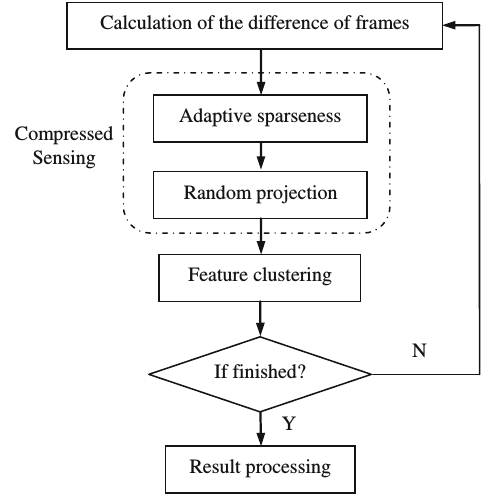
\includegraphics[scale=0.4]{figure/flow.png}
        \end{column}
    \end{columns}
\end{frame}


\begin{frame}{入力データ形式}
\begin{block}{データの変換}
\begin{itemize}
 \item $I$ : 現在のフレーム
 \item $\Delta I$ : $I$ と背景フレームとの差分
 \item $I'$ : K-SVDの入力,下記の変換をかけた $\Delta I$
\end{itemize}
\end{block}
$h_a * h_a$ サイズのブロック列化
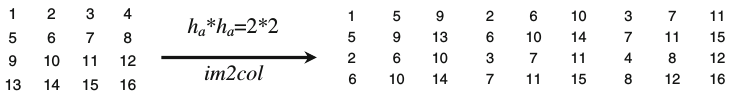
\includegraphics[scale=0.5]{figure/im2col.png}
\end{frame}


\begin{frame}{Adaptive sparseness}
カメラのノイズなど余分な情報を K-SVD で圧縮

\begin{block}{アルゴリズム}
\begin{enumerate}
    \item 入力 (p. \ref{ksvd} の $Y$) を $I'$ とする
    \item 辞書 $D$ の DCT 行列による初期化
    \item OMP により $D$ を反復最適化
    \item 得られた疎表現 (p. \ref{ksvd} の $X$) を $I_{sparse}$ とする
\end{enumerate}
\end{block}
    \begin{columns}
        \begin{column}{0.2\textwidth} % 右:40%
            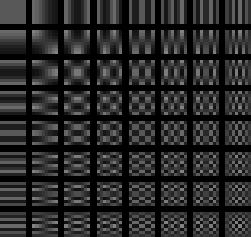
\includegraphics[height=2cm]{figure/dct.png}
        \end{column}
        \begin{column}{0.8\textwidth} % 左:60%
        DCT (下記) の高周波成分はほぼ 0 なので疎表現
        \begin{eqnarray}
            D_{1,j} & = & 1 / \sqrt{N} \\
            D_{i,j} & = & \sqrt{2/N} \cos{\frac{\pi (2j - 1) (i + 1)}{2 N}}
        \end{eqnarray}
        \end{column}
    \end{columns}

\end{frame}



\begin{frame}{Random projection}
疎表現 $I_{sparse}$ をさらに低次元へ圧縮
\begin{eqnarray}
    I_{feature} & = & \rproSymbol I_{sparse}
\end{eqnarray}
ここで $\rproSymbol \in \rsize{M \times N}$ は measurement matrix と呼ばれる.
\begin{block}{measurement matrix}
$\rproSymbol$ は入力が疎なら random Gaussian matrix を用いると比較的良い性能が知られる (RIP を調べなくても良い)\cite{Candes2006}
\end{block}
筆者らは$\mathrm{Norm}(0, 1/M)$ を用いた.
また $M$ は不等式
\begin{equation}
    M \geq c K \log{N/K}
\end{equation}
に基づき経験的に決めた.$K$ は sparseness, $c$ は小さな定数(?!).
\end{frame}


\begin{frame}{Main working steps}
\begin{enumerate}
    \item $I'$ : 現時刻における差分フレームの $3\times3$ ブロック表現
    \item $I_{sparse}$ : K-SVD による $I'$ の疎表現
    \item $I_{feature}$ : Gaussian Matrix による3次元への圧縮 $\rproSymbol I_{sparse}$
    \item $\Lambda$ : K-Means による$I_{feature}$ の二値化
    \item $I_{result}$ : 近傍フレームの $\Lambda$ の論理和に Erosion と Dilation
\end{enumerate}
以上を 5 フレームおきに処理
\end{frame}
